% !TEX TS-program = xelatex
% !TEX encoding = UTF-8 Unicode
% !Mode:: "TeX:UTF-8"

\documentclass{resume}
\usepackage{zh_CN-Adobefonts_external} % Simplified Chinese Support using external fonts (./fonts/zh_CN-Adobe/)
%\usepackage{zh_CN-Adobefonts_internal} % Simplified Chinese Support using system fonts
\usepackage{linespacing_fix} % disable extra space before next section
\usepackage{cite}
\setstretch{1.08} % slightly increase overall line spacing while keeping one-page layout


% \documentclass{resume}
% \usepackage{graphicx}
% \usepackage{zh_CN-Adobefonts_external}
% \usepackage{linespacing_fix}
% \usepackage{cite}



\begin{document}
\pagenumbering{gobble} % suppress displaying page number

% \name{杜靖怡}

% \contactInfo{(+86) 185-3792-2003}{dujingyi7714@163.com}
% {GitHub @hijiangtao}

\vspace*{-0.35\baselineskip}
\noindent
\begin{tabular*}{\textwidth}{@{}p{0.22\textwidth}@{}p{0.56\textwidth}@{}p{0.22\textwidth}@{}}
    &
    \begin{minipage}[b]{0.56\textwidth}
        \centering
        {\Huge \textbf{杜靖怡}}
        
        \vspace{0.8\baselineskip}
        \mbox{\small 电话：18537922003\hspace{0.8em}邮箱：dujingyi7714@163.com}
    \end{minipage}
    &
    \begin{minipage}[b]{0.22\textwidth}
        \raggedleft
        \raisebox{-1.5\baselineskip}[0pt][0pt]{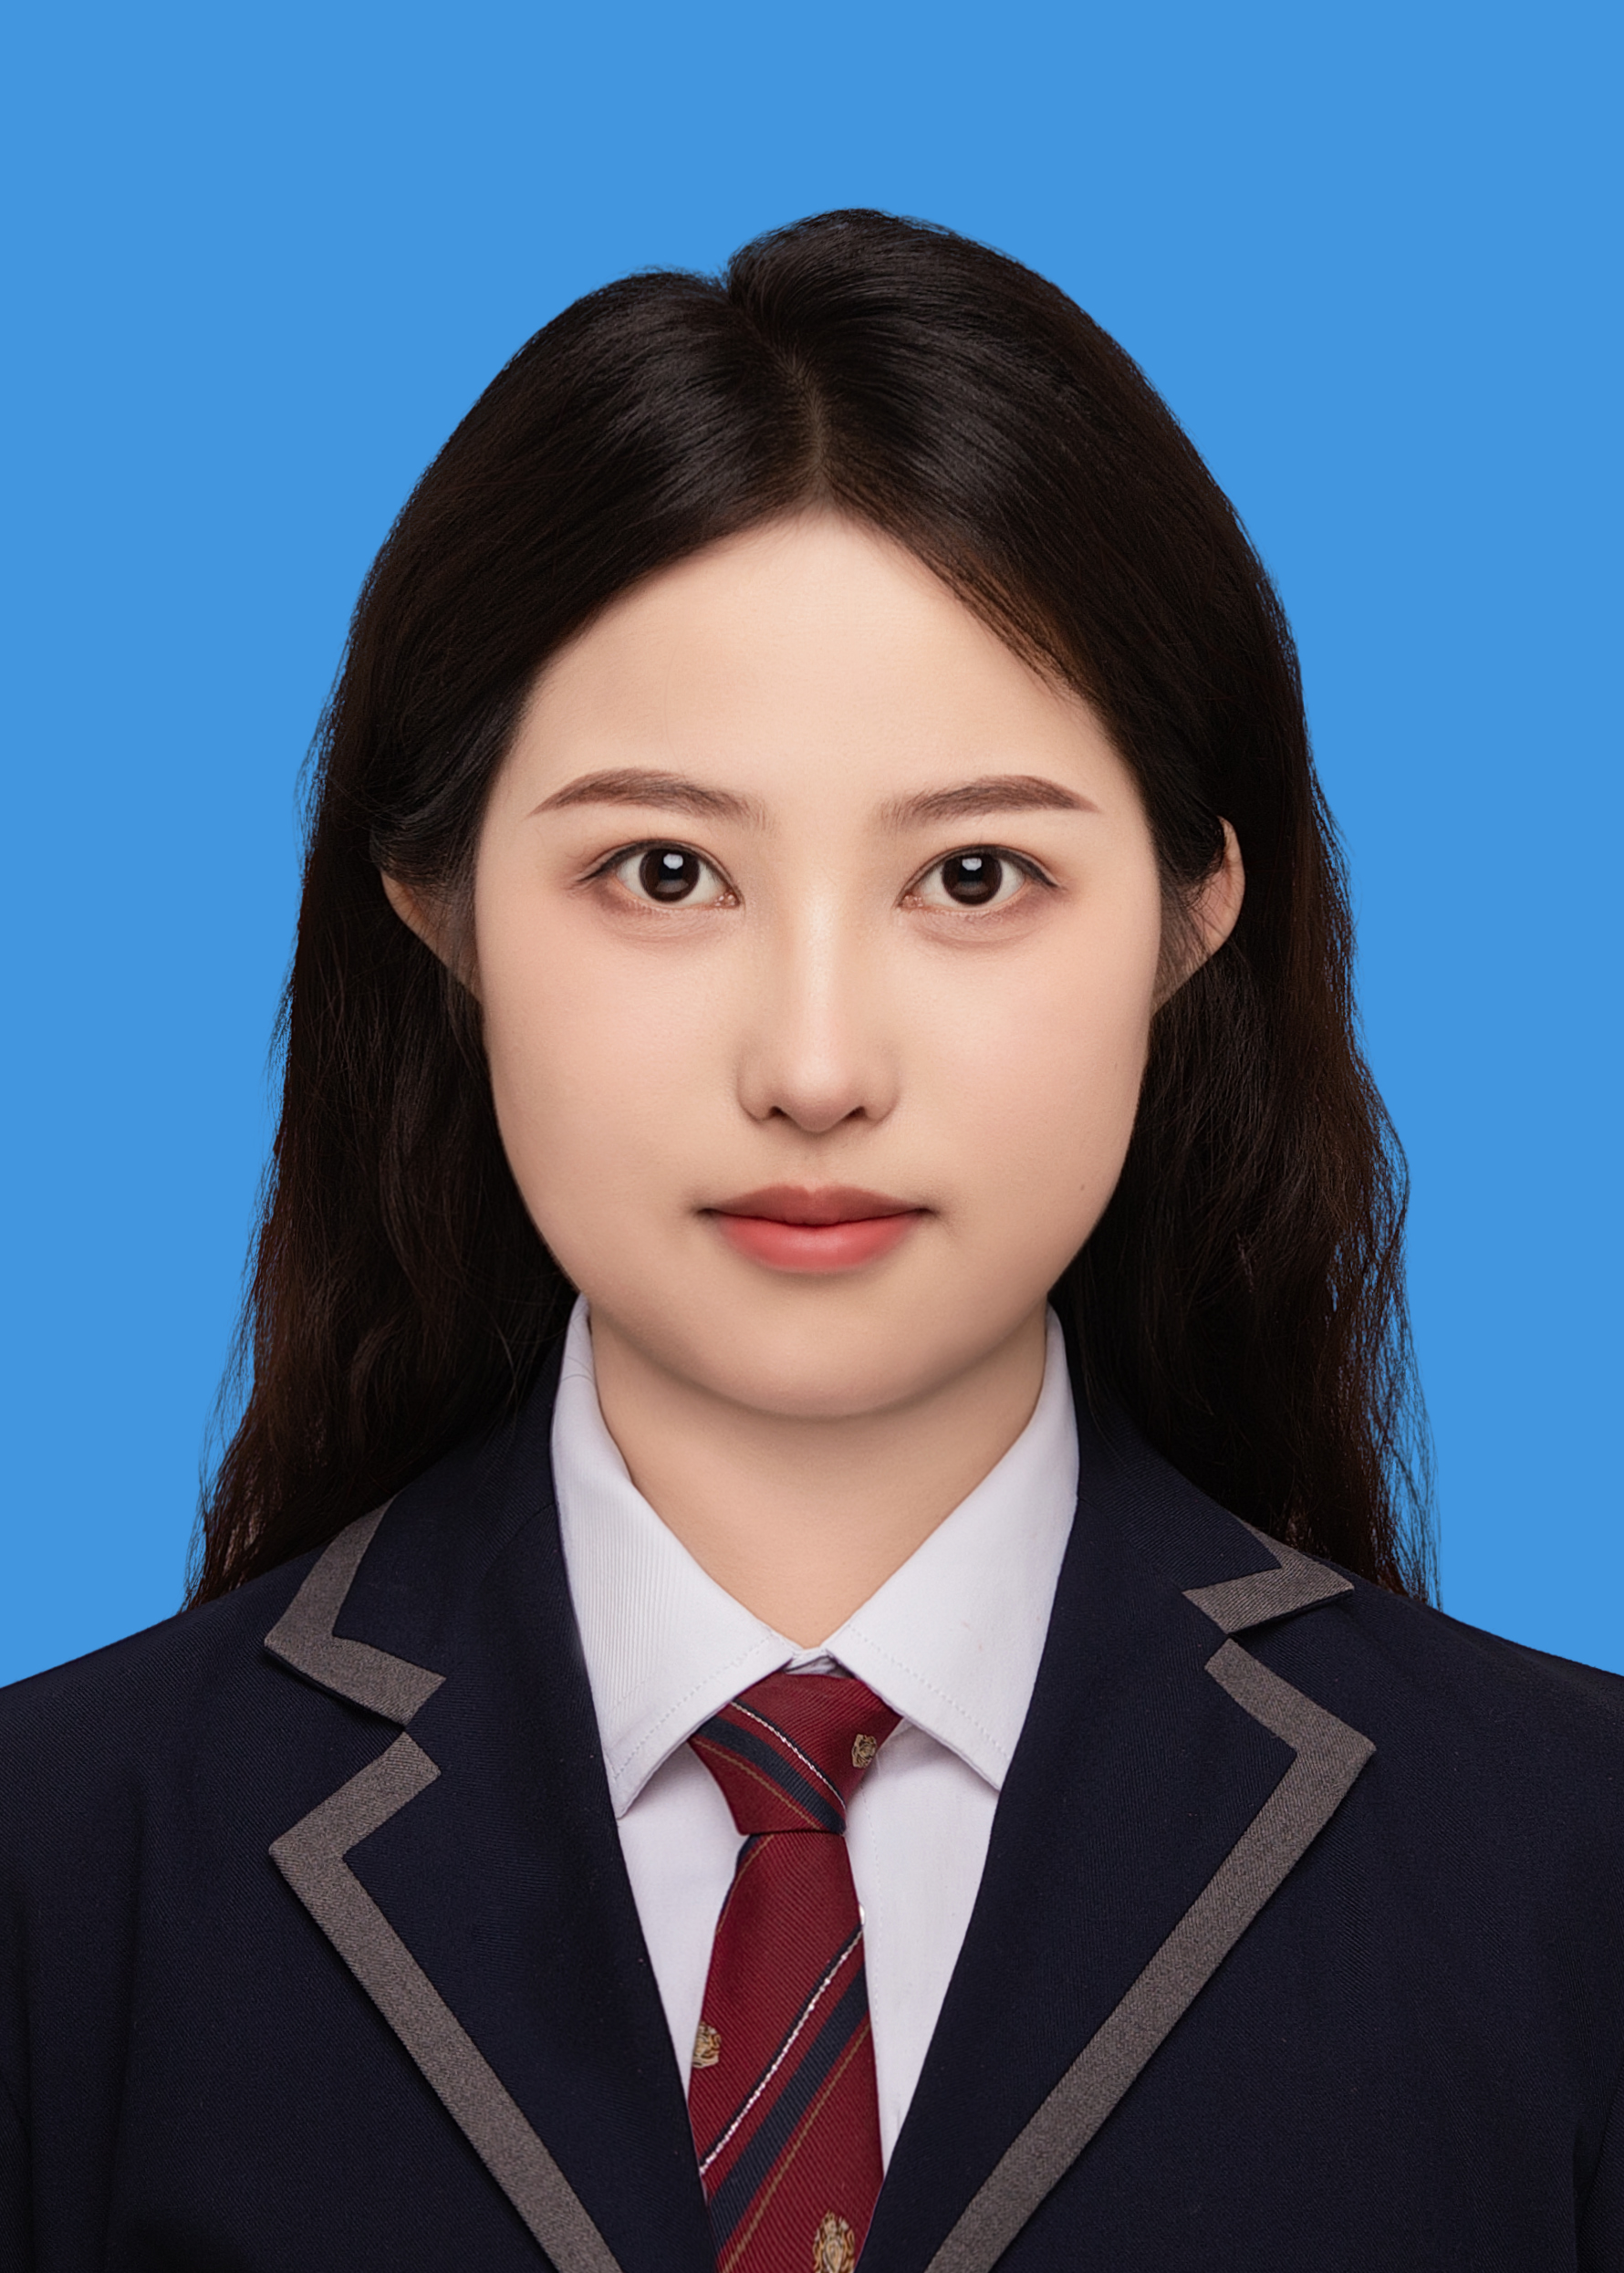
\includegraphics[width=2.5cm]{photo.jpg}}
    \end{minipage}
\end{tabular*}

\vspace{0.5\baselineskip}





\section{教育经历}

{
\renewcommand{\arraystretch}{1.25}
\begin{tabular*}{\textwidth}{@{\extracolsep{\fill}} l l l r}
\textbf{吉林大学(985)} & 统计学 & 硕士在读 & 2025.09 - 2028.06 \\
\textbf{湘潭大学(双一流)} & 统计学 & 理学学士 & 2021.09 - 2025.06 \\
\end{tabular*}
}

\vspace{-0.8em}

\begin{itemize}
    \item \textbf{GPA}: 3.34/4.0 \hfill \textbf{CET4}: 566 \hfill \textbf{CET6}: 520 \hfill \textbf{雅思}: 6.5
    \item \textbf{主修课程}：概率论与数理统计、机器学习、深度学习、时间序列分析、运筹与优化、多元统计分析
    \item \textbf{奖项/荣誉}： 全国大学生数学建模竞赛省一、统计建模大赛省二、校级三好学生、湖南省优秀毕业生
  
\end{itemize}

\section{项目经历}



\datedsubsection{\textbf{多行为序列建模的 OTTO 电商推荐与用户行为预测}}{2026.05-2026.06}
\begin{itemize}

  \item 面向 OTTO 电商行为数据构建 \textbf{clicks/carts/orders 多目标推荐任务}，处理约 \textbf{6014 万条训练日志、208 万条验证日志、45 万个 session}，完成数据清洗、行为编码与验证集构造。

  \item 设计 \textbf{Item-to-Item 共现召回策略}，融合 \textbf{clicks、carts-orders、buy2buy 三类共现矩阵}，结合\textbf{行为权重 1:5:4、时间窗口和时间衰减} 生成候选商品。

  \item 构造商品侧、session 侧、session-aid 交互侧共 \textbf{37 维排序特征}，生成约 \textbf{6755 万条候选样本}，并通过\textbf{分片存储和负采样} 缓解内存压力与样本不平衡问题。

  \item 使用 \textbf{XGBoost} 分别训练三类排序模型，并以 session 为 group 采用 \textbf{GroupKFold} 进行交叉验证，本地验证集达到 \textbf{Weighted Recall@20 = 0.5410}，其中 orders 任务 \textbf{Recall@20 = 0.6234}。

\end{itemize}





\datedsubsection{\textbf{个人信用违约风险预测与阈值优化模型}}{2026.04-2026.05}
\begin{itemize}

  \item 面向金融风控中\textbf{违约客户识别}场景，针对 German Credit 数据集存在类别不均衡、违约样本占比仅约 \textbf{30\%} 的问题，完成类别变量编码与特征处理，将原始数据整理为 \textbf{1000 条样本、38 维特征}，并采用分层抽样按 \textbf{600 / 200 / 200} 划分训练集、验证集和测试集，保证各数据集类别比例一致。

  \item 选择 \textbf{Logistic Regression、Random Forest、SVM、GBDT、XGBoost} 五个模型，使用 \textbf{Stratified 5-Fold CV + GridSearchCV} 完成超参数搜索，共评估101 组参数组合、505 次模型训练；以 \textbf{ROC-AUC} 作为主优化指标进行模型对比，最优模型在测试集上达到 \textbf{0.7952}。

  \item 针对信用风控中\textbf{漏判违约客户成本较高}的问题，在验证集上为各参数最优模型搜索 \textbf{KS 最大化阈值}，并在测试集上对比默认阈值0.5与 KS 阈值下的分类效果；其中 SVM 的违约召回率由 \textbf{46.7\%} 提升至 \textbf{86.7\%}，漏判数由 \textbf{32} 降至 \textbf{8}，显著提升了模型对高风险客户的捕捉能力。

\end{itemize}
    

\datedsubsection{\textbf{量子卷积特征提取的混合经典-量子图像分类}}{2025.11-2025.12}
\begin{itemize}

  \item 使用\textbf{Fashion-MNIST}数据集构建 Classical CNN 与 Quantum-enhanced CNN 对照实验，处理 \textbf{28$\times$28 灰度图像、10 类样本}，对10000张图像完成预处理、二值化编码、量子特征生成与模型评估。

  \item 基于 \textbf{PyTorch} 搭建 \textbf{2 层 Conv2d-BatchNorm-ReLU-MaxPool + 全连接层} 的 CNN 分类器，使用 \textbf{CrossEntropyLoss + Adam} 训练；随机生成 \textbf{5 个量子电路}，将原始 \textbf{1 通道图像} 转换为 \textbf{5 通道量子特征图}，并在相同分类器结构下对比。

  \item 经典 CNN 测试准确率\textbf{80.4\%}，量子增强模型在测试集上的分类准确率为\textbf{82.3\%}，实验结果表明量子电路能够完成有效图像表征。
  
\end{itemize}


% \section{\faCogs\ IT 技能}
\section{专业技能}
% increase linespacing [parsep=0.5ex]
\begin{itemize}[parsep=0.2ex]
  \item \textbf{编程与数据处理}: 熟悉 Python 和 R，具备数据清洗、特征工程、实验分析和模型评估能力；了解 SQL、Git、Linux 基础操作；能够熟练使用Codex、Claude Code等AI开发工具。
  \item \textbf{机器学习与深度学习}: 掌握 决策树、随机森林、GBDT、XGBoost 等机器学习算法，熟悉交叉验证、特征选择、类别不平衡处理和模型调参方法；熟悉 PyTorch 框架，了解 MLP、CNN、RNN/LSTM、Transformer 等深度学习模型结构，具备复现和调试能力。

  \item \textbf{数理统计基础}:具备扎实的概率论、数理统计、回归分析、时间序列分析和运筹优化基础；熟悉假设检验、ARIMA、非线性规划等方法，具备统计建模、预测分析和业务问题抽象能力。
\end{itemize}

% \section{\faHeartO\ 项目/作品摘要}
% \section{项目/作品摘要}
% \datedline{\textit{An Integrated Version of Security Monitor Vis System}, https://hijiangtao.github.io/ss-vis-component/ }{}
% \datedline{\textit{Dark-Tech}, https://github.com/hijiangtao/dark-tech/ }{}
% \datedline{\textit{融合社交网络数据挖掘的电视节目可视化分析系统}, https://hijiangtao.github.io/variety-show-hot-spot-vis/}{}
% \datedline{\textit{LeetCodeOJ Solutions}, https://github.com/hijiangtao/LeetCodeOJ}{}
% \datedline{\textit{Info-Vis}, https://github.com/ISCAS-VIS/infovis-ucas}{}




%% Reference
%\newpage
%\bibliographystyle{IEEETran}
%\bibliography{mycite}
\end{document}
